\documentclass[portrait,a0paper,fontscale=0.4]{baposter}

% Packages for input encoding and localization
\usepackage[utf8]{inputenc}
\usepackage[english]{babel}

\usepackage[font=small,labelfont=bf]{caption}
\usepackage{float}
\usepackage{relsize} % http://ftp.gwdg.de/pub/ctan/macros/latex/contrib/relsize/relsize-doc.pdf
\usepackage{tcolorbox}
\usepackage{textcomp}

\definecolor{azure}{rgb}{0.0, 0.5, 1.0}
\definecolor{babyblueeyes}{rgb}{0.63, 0.79, 0.95}
\definecolor{blue-violet}{rgb}{0.54, 0.17, 0.89}
% Package for better URL support
\usepackage{url}

% Package to include graphics
\usepackage{graphicx}
\graphicspath{{./fig/}}
\DeclareGraphicsExtensions{.png,.pdf,.jpg,.jpeg}
\usepackage{subfig}
\usepackage{enumitem}

\setlength{\abovecaptionskip}{-5pt}

\usepackage{palatino}
% Package for program listings
\usepackage{listings}
% Settings for the listings package
\lstset{
  language=C,
  emphstyle={\em},
  }

% Packages for nicer tables
\usepackage{tabularx}
\usepackage{multirow}
\usepackage{booktabs} % for tables
\captionsetup[figure]{labelformat=simple,skip=0.75em,name=Fig.}

\newcommand{\tabularTextSize}[0]{\tiny}
\newcommand{\mycomment}[1]{}
\newcommand{\verytiny}{\fontsize{4}{12} \selectfont \setlength{\baselineskip}{4pt plus 2pt minus 1pt}}
\newcommand{\compresslist}{%
\setlength{\itemsep}{1pt}%
\setlength{\parskip}{0pt}%
\setlength{\parsep}{0pt}%
}


\begin{document}
  \definecolor{UHAM}{HTML}{e30613} %87CEEB
  \definecolor{UHAMLight}{HTML}{e37673} %87CEEB


  % % Setting the watermark image
  % \background
  % {
  %     \begin{tikzpicture}[remember picture,overlay]%
  %     \draw (current page.center) node[opacity=0.3]
  %       {\includegraphics[scale=5]{SIOX-Logo}};
  %     \end{tikzpicture}%
  % }

\begin{poster}
{ % key=value option
  grid=false,
  columns = 4,
  eyecatcher=true,
  background=shadeTB,%user
  bgColorOne=white,
  bgColorTwo=white,
  borderColor=UHAM,
  headerColorOne=UHAMLight,
  headerColorTwo=UHAMLight,%white
  headershape=rounded,
  headerheight=4.8cm,
  textfont={\setlength{\parindent}{0em} \setlength{\parskip}{0.75em}},
  headerborder=open,
  textborder=rounded,
  boxshade=plain,%shadeTB
  boxColorOne=white,
  boxColorTwo=UHAM
}{ % Eye Catcher
  \begin{minipage}{0.2\textwidth}
   \begin{center}
    
\includegraphics[width=0.8\textwidth]{logo-io500.pdf}
   \end{center}
  \end{minipage}

}{ % Poster Title
  \textbf{The Virtual Institute for I/O and the IO-500}
  %\medskip
  %\textbf{\huge xx}
}{ % Poster Authors
  \vspace{0.5em}
  \textsc
  Julian Kunkel$^1$, Jay Lofstead$^2$, John Bent$^3$
  \\[0.5em]
  \emph{$^1$ Deutsches Klimarechenzentrum (DKRZ)}
  \hspace*{2em}
  \emph{$^2$ Sandia National Laboratory}
   \hspace*{2em}
  \emph{$^3$ Cray}
  \\[0.5em]
   Contact: \url{juliankunkel@gmail.com}
}{
    \begin{minipage}{0.2\textwidth}
     \begin{center}
      
\includegraphics[width=0.8\textwidth]{logo-vi4io.png}
     \end{center}
    \end{minipage}
}


\begin{posterbox}[name=problem,column=0]
{Introduction}

The research community in high-performance computing is organized loosely.
There are many distinct resources such as homepages of research groups and benchmarks.
The Virtual Institute for I/O aims to provide a hub for the community and particularly newcomers to find relevant information in many directions.
Additionally, we host the \textbf{comprehensive data center list (CDCL)}. Similarly to the top500, it contains information about supercomputers and their storage systems.
Additionally, in the community, we are working on standardizing an I/O benchmark.

This poster introduces the Virtual Institute for I/O, the high-performance storage list and the effort for the IO-500 which are unfunded community projects.
\end{posterbox}


\begin{posterbox}[name=approach,column=0,below=problem]
{The Virtual Institute for I/O}


Goals of the Virtual Institute for I/O (VI4IO) are
\vspace*{-1em}
\begin{itemize}\compresslist
\item Provide a platform for I/O researchers and enthusiasts for exchanging information
\item Foster training and international collaboration in the field of high-performance I/O
\item Track/encourage the deployment of large storage systems by hosting information about high-performance storage systems
\end{itemize}
\vspace*{-1em}

The philosophical cornerstones of VI4IO are:

\vspace*{-1em}
\begin{itemize}\compresslist
\item Treat contributors/participants equally
\item Allow free participation without any fee inclusive to all
\item Independent of vendors/research facilities
\end{itemize}
\end{posterbox}


\begin{posterbox}[name=overview,column=0,below=approach]{Open Organization}

The organization uses a wiki as central hub
\vspace*{-1em}
\begin{itemize}\compresslist
\item Registered users can edit the content
\item Mayor changes should be discussed on the contribute mailing list
\item Tag clouds link between similar entities
\item Supported by mailing lists, e.g.:
\begin{itemize}\compresslist
\item Call-for-papers
\item Announcements
\item Contributions / suggestions
\end{itemize}
\end{itemize}

\end{posterbox}


\begin{posterbox}[name=wps,column=0,below=overview]{CDCL System Model}
The comprehensive data center list with its system model describes how characteristics are assigned to components.
Storage is difficulty to assign to a single component as it is often shared across supercomputers,
therefore, a flexible component based model is used.

Supported components:
\vspace*{-1em}
\begin{itemize}\compresslist
\item Site: Describes the facility
\item Supercomputer: A system
\item Storage system
\item Nodes
\item Network
\item Building
\end{itemize}

\vspace*{-1em}

The schema is under active development -- we aim to describe data center characteristics.
The web page allows the creation of a topology for the facility to indicate the relation between the components -- ultimately multiple views will be created.
\end{posterbox}

\begin{posterbox}[name=io500res,column=0,above=bottom,below=wps]{IO-500 List Nov 2017}
  
\includegraphics[width=\textwidth]{logo-io500.pdf}

  \vspace*{1em}
  
  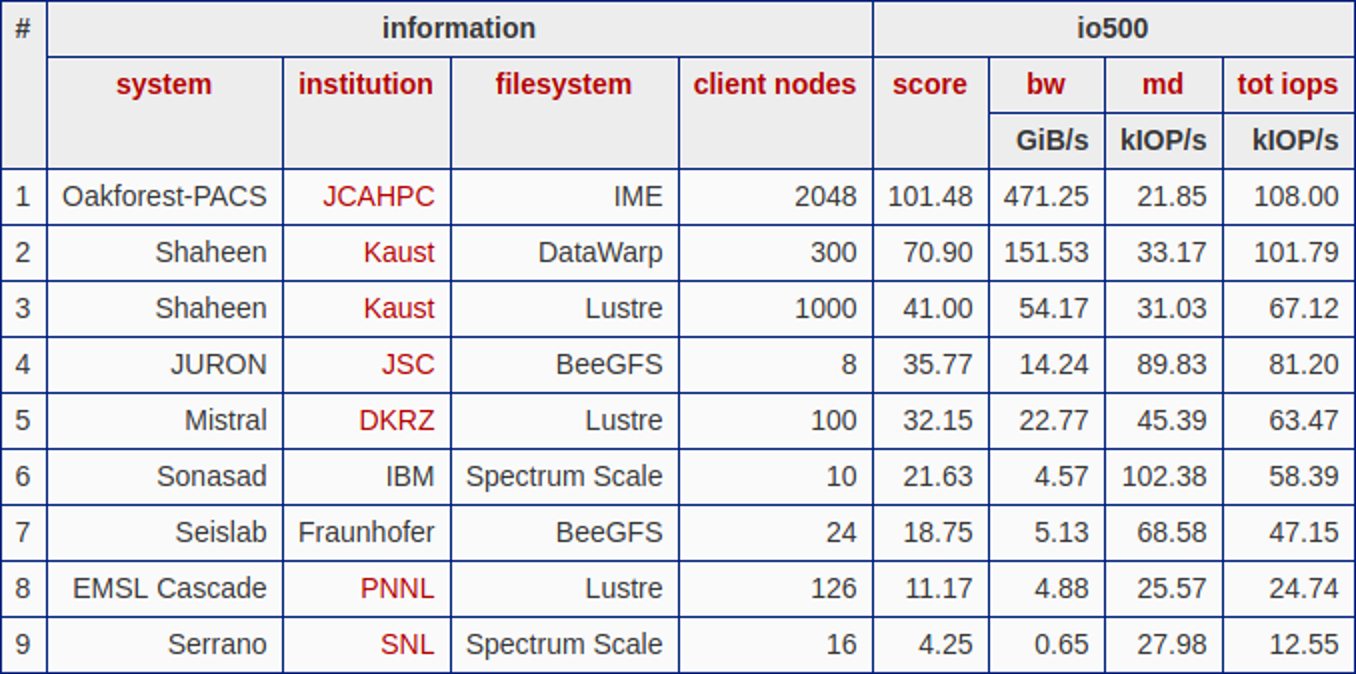
\includegraphics[width=\textwidth]{io500}
\end{posterbox}


%%%%%%%%%%%%%%%%%%%%%%%%%%%%%%%%%%%%%%%%%%%%%%%%%%%%%%%
\begin{posterbox}[name=concept,column=1,span=2]{Community Content of the VI4IO Wiki}
\begin{minipage}{7cm}
Worldwide research groups that address high-performance I/O including:

\vspace*{-1em}
\begin{itemize}\compresslist
\item A taglist for available knowledge
\item Research products such as file systems
\item Ongoing research projects
\end{itemize}

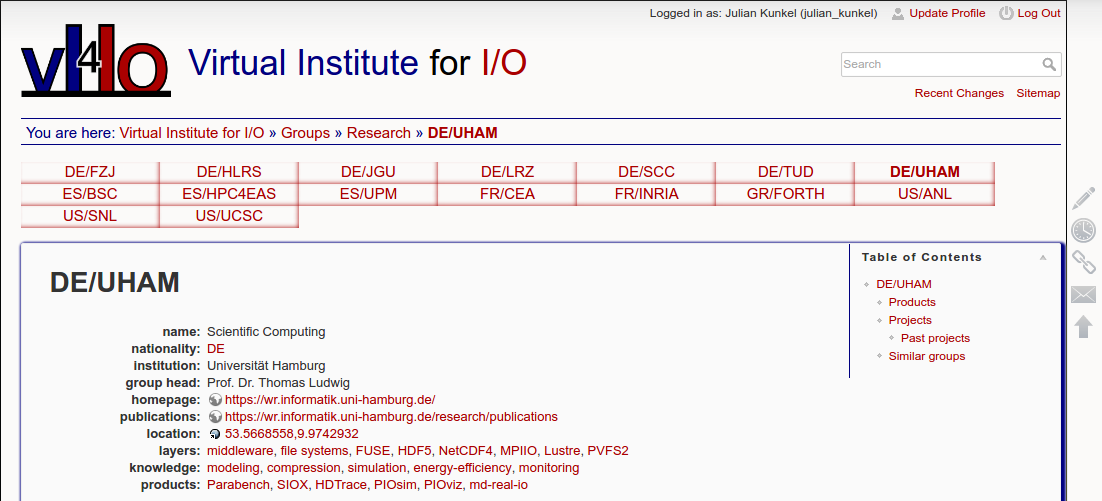
\includegraphics[width=7.5cm]{groups}

Everyone is welcome to add (own) group(s)!

\end{minipage}
\hfill
\begin{minipage}{7.5cm}

Relevant I/O related tools and benchmarks.

\vspace*{1em}

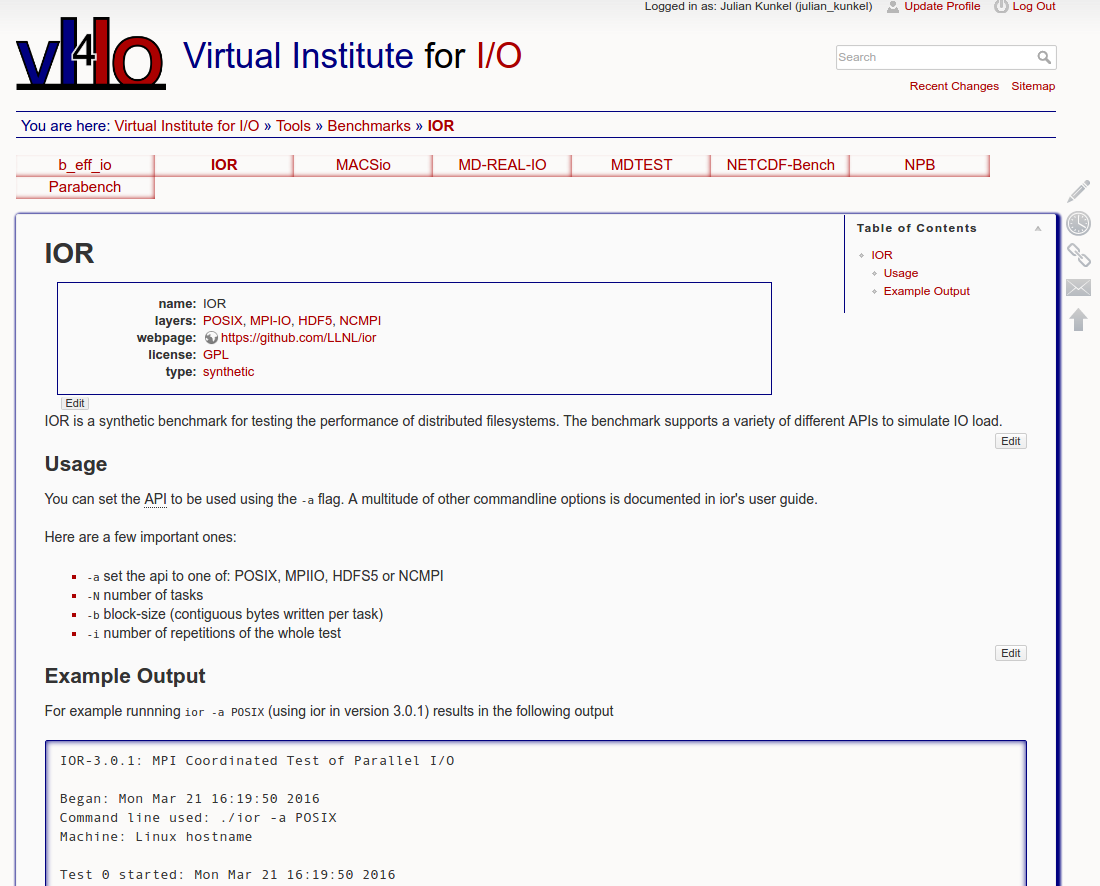
\includegraphics[width=7cm]{benchmark}
\end{minipage}
\end{posterbox}


\begin{posterbox}[name=schedule,column=1,span=2, below=concept]{High-Performance Storage List}
The High-Performance storage list contains the characteristics of site, supercomputer and connected storage (see the box about the system model).
The list shown in the box on the right is sortable on the metric of choice.
It allows to add/remove metrics (see the list next).
Graphs are created based on selectable grouping.


\textbf{Metrics:} Most metrics can be determined without measurement and describe hardware and software characteristics that should be well known to the site and vendor. A few metrics cover actually observed metadata and I/O performance, in this case the measurement procedure must be clear.
The list stores data entered in the wiki into a database and converts data to a base unit.

The following list of supported metrics includes a description:

\begin{minipage}{0.48\textwidth}
\textbf{Institution}
\scriptsize
\begin{itemize}\compresslist
\item institution: The abbreviation of the institution. Note that systems are linked together based on year and institution.
\item year: The year for which the data is valid.
\item nationality: The international abbreviation for the nationality of the institution.
\item web page: The web page of the institution.
\item energy consumption: The overall energy consumption of the datacenter.
\item power usage effectiveness: The PUE of the datacenter.
\end{itemize}

\normalsize
\textbf{Supercomputer}
\scriptsize\begin{itemize}\compresslist
\item institution: see above
\item year:  see above
\item vendor: The vendor of the supercomputer.
\item software: A list of keywords with relevant software components, e.g., which file system, parallelization software.
\item installation: This is the date when the supercomputer has been installed. Multi-phase installations should appear with their last upgrade date.
\item compute peak: The theoretical peak performance in FLOPs.
\item node count: The number of nodes.
\item total cores: The total number of available cores.
\item memory capacity: The available memory capacity in Bytes.
\item memory bandwidth: The sum of the theoretical memory bandwidth available in B/s.
\item memory per node: The memory capacity per node.
\item application domain: A list of the main (scientific) domains that use this supercomputer.
\item applications: A list of the main applications (if known).
\item energy consumption: The energy consumption of the supercomputer (without storage) in Watts – this does not take the PUE into account.
\item interconnect: A list of keywords about the interconnect.
\item processor: A list of keywords specifying the processor.
\item graph500: The achieved performance according to the graph 500 list. This is not the position in the list, as this may change over time.
\item graph500 problem scale: according to the graph 500 list.
\item top500: The achieved performance according to the top 500.
\item green500: The achieved efficiency according to the green 500.
\item architecture: A list of keywords covering the system architecture, e.g., i386 64, GPGPU
\end{itemize}
\end{minipage}
\quad
\begin{minipage}{0.48\textwidth}


\textbf{Storage}

{
\scriptsize
\begin{itemize}\compresslist
\item institution:  see left
\item year:  see left
\item type: The type of the storage, i.e., tape archive/shared storage
\item installation: see left
\item energy consumption: The energy consumption of the storage part in Watts – this does not take the PUE into account.
\item capacity: The effective capacity that is available to users. It includes overhead of erasure (RAID) coding and potential hot/cold spares. This value can be easily derived from the number of available storage devices that support the listed file system.
\item interconnect: A list of keywords about the interconnect.
\item drives: The total number of tape drives for a nearline tape/MAID archive.
\item cache size: The amount of storage cache in a nearline HSM.
\item slots: The number of slots in a nearline tape/MAID archive to hold media.
\item vendor: The vendor of the storage hardware.
\item software: A list of keywords specifying the software further.
\item hardware: A list of keywords specifying the hardware further.
\item peak: The theoretical peak performance of the storage system. The value is the performance that could theoretically be achieved when transferring data between clients and storage. It is limited by 1) the aggregated network throughput between client and servers, 2) the aggregated (RAID) controller throughput, 3) the network topology.
\item \textit{metadata rate}: Metadata throughput. The value can be determined using any I/O benchmark of choice that ensures that client-side and server-side caches are overwhelmed.
\item \textit{sustained write}: Best I/O throughput ever measured when accessing files. The read and write values can be determined using any I/O benchmark of choice that ensures that client-side and server-side caches are overwhelmed.
\item \textit{sustained read}: (see the description for write)
\item servers: The number of storage servers of the storage system.
\item hdds: The number of HDDs that belong to the storage system.
\item ssds: The number of SSDs that belong to the storage system.
\end{itemize}
}
\end{minipage}

\textbf{Measurement procedure for sustained performance:}
Compared to other lists (TOP500, Green500) that have a clear measurement process, the rules for determining sustained performance for the HPSL are relaxed due to the complexity of I/O benchmarks, However it must be clarified how the measurement has been conducted.
\end{posterbox}

\begin{posterbox}[name=HHCC,column=1,span=2, below=schedule, above=bottom]{IO-500 Effort}
We are discussing the creation of a benchmark to compare facilities and storage systems. This challenge is explored on our task page: \url{http://www.io500.org} and mailing list.

\textbf{Goals for the benchmark:}

\vspace*{-0.5em}

\begin{minipage}{10.5cm}
\begin{itemize}
\item Capture user-experienced performance % and honor system balance
\item Reported performance is representative for:
\vspace*{-0.5em}
\begin{itemize}
\item IOEasy: Applications with well optimized I/O patterns
\item IOHard: Applications that require a random workload
\item IOMD: Usage that depends on metadata/small objects
\end{itemize}
\end{itemize}
\end{minipage}
\qquad
\begin{minipage}{4cm}

\includegraphics[width=3.8cm]{border}
\end{minipage}
%\qquad
%\begin{minipage}{6cm}
%x
%\end{minipage}

\vspace*{-1em}

Challenges:
\vspace*{-1em}
\begin{itemize}
\item Representative: for optimized, naive I/O heavy workloads; and small objects
\item Inclusive: cover various storage technology and non-POSIX APIs
\item Trustworthy: representative results and prevent cheating
\item Cheap: easy to run and short benchmarking time (in the order of minutes)
\end{itemize}


Strategy:
\vspace*{-1em}
\begin{itemize}
\item Build on existing benchmarks
\item Plugin systems should allow for alternative storage technology
\item Start by reporting one metric per benchmark, decide later about a single number
\end{itemize}


\end{posterbox}



%%%%%%%%%%%%%%%%%%%%%%%%%%%%%%%%%%%%%%%%%%%%%%%%%%%%%%%



\begin{posterbox}[name=engineering,column=3]{HPSL 2018}
The current list contains 39 sites:

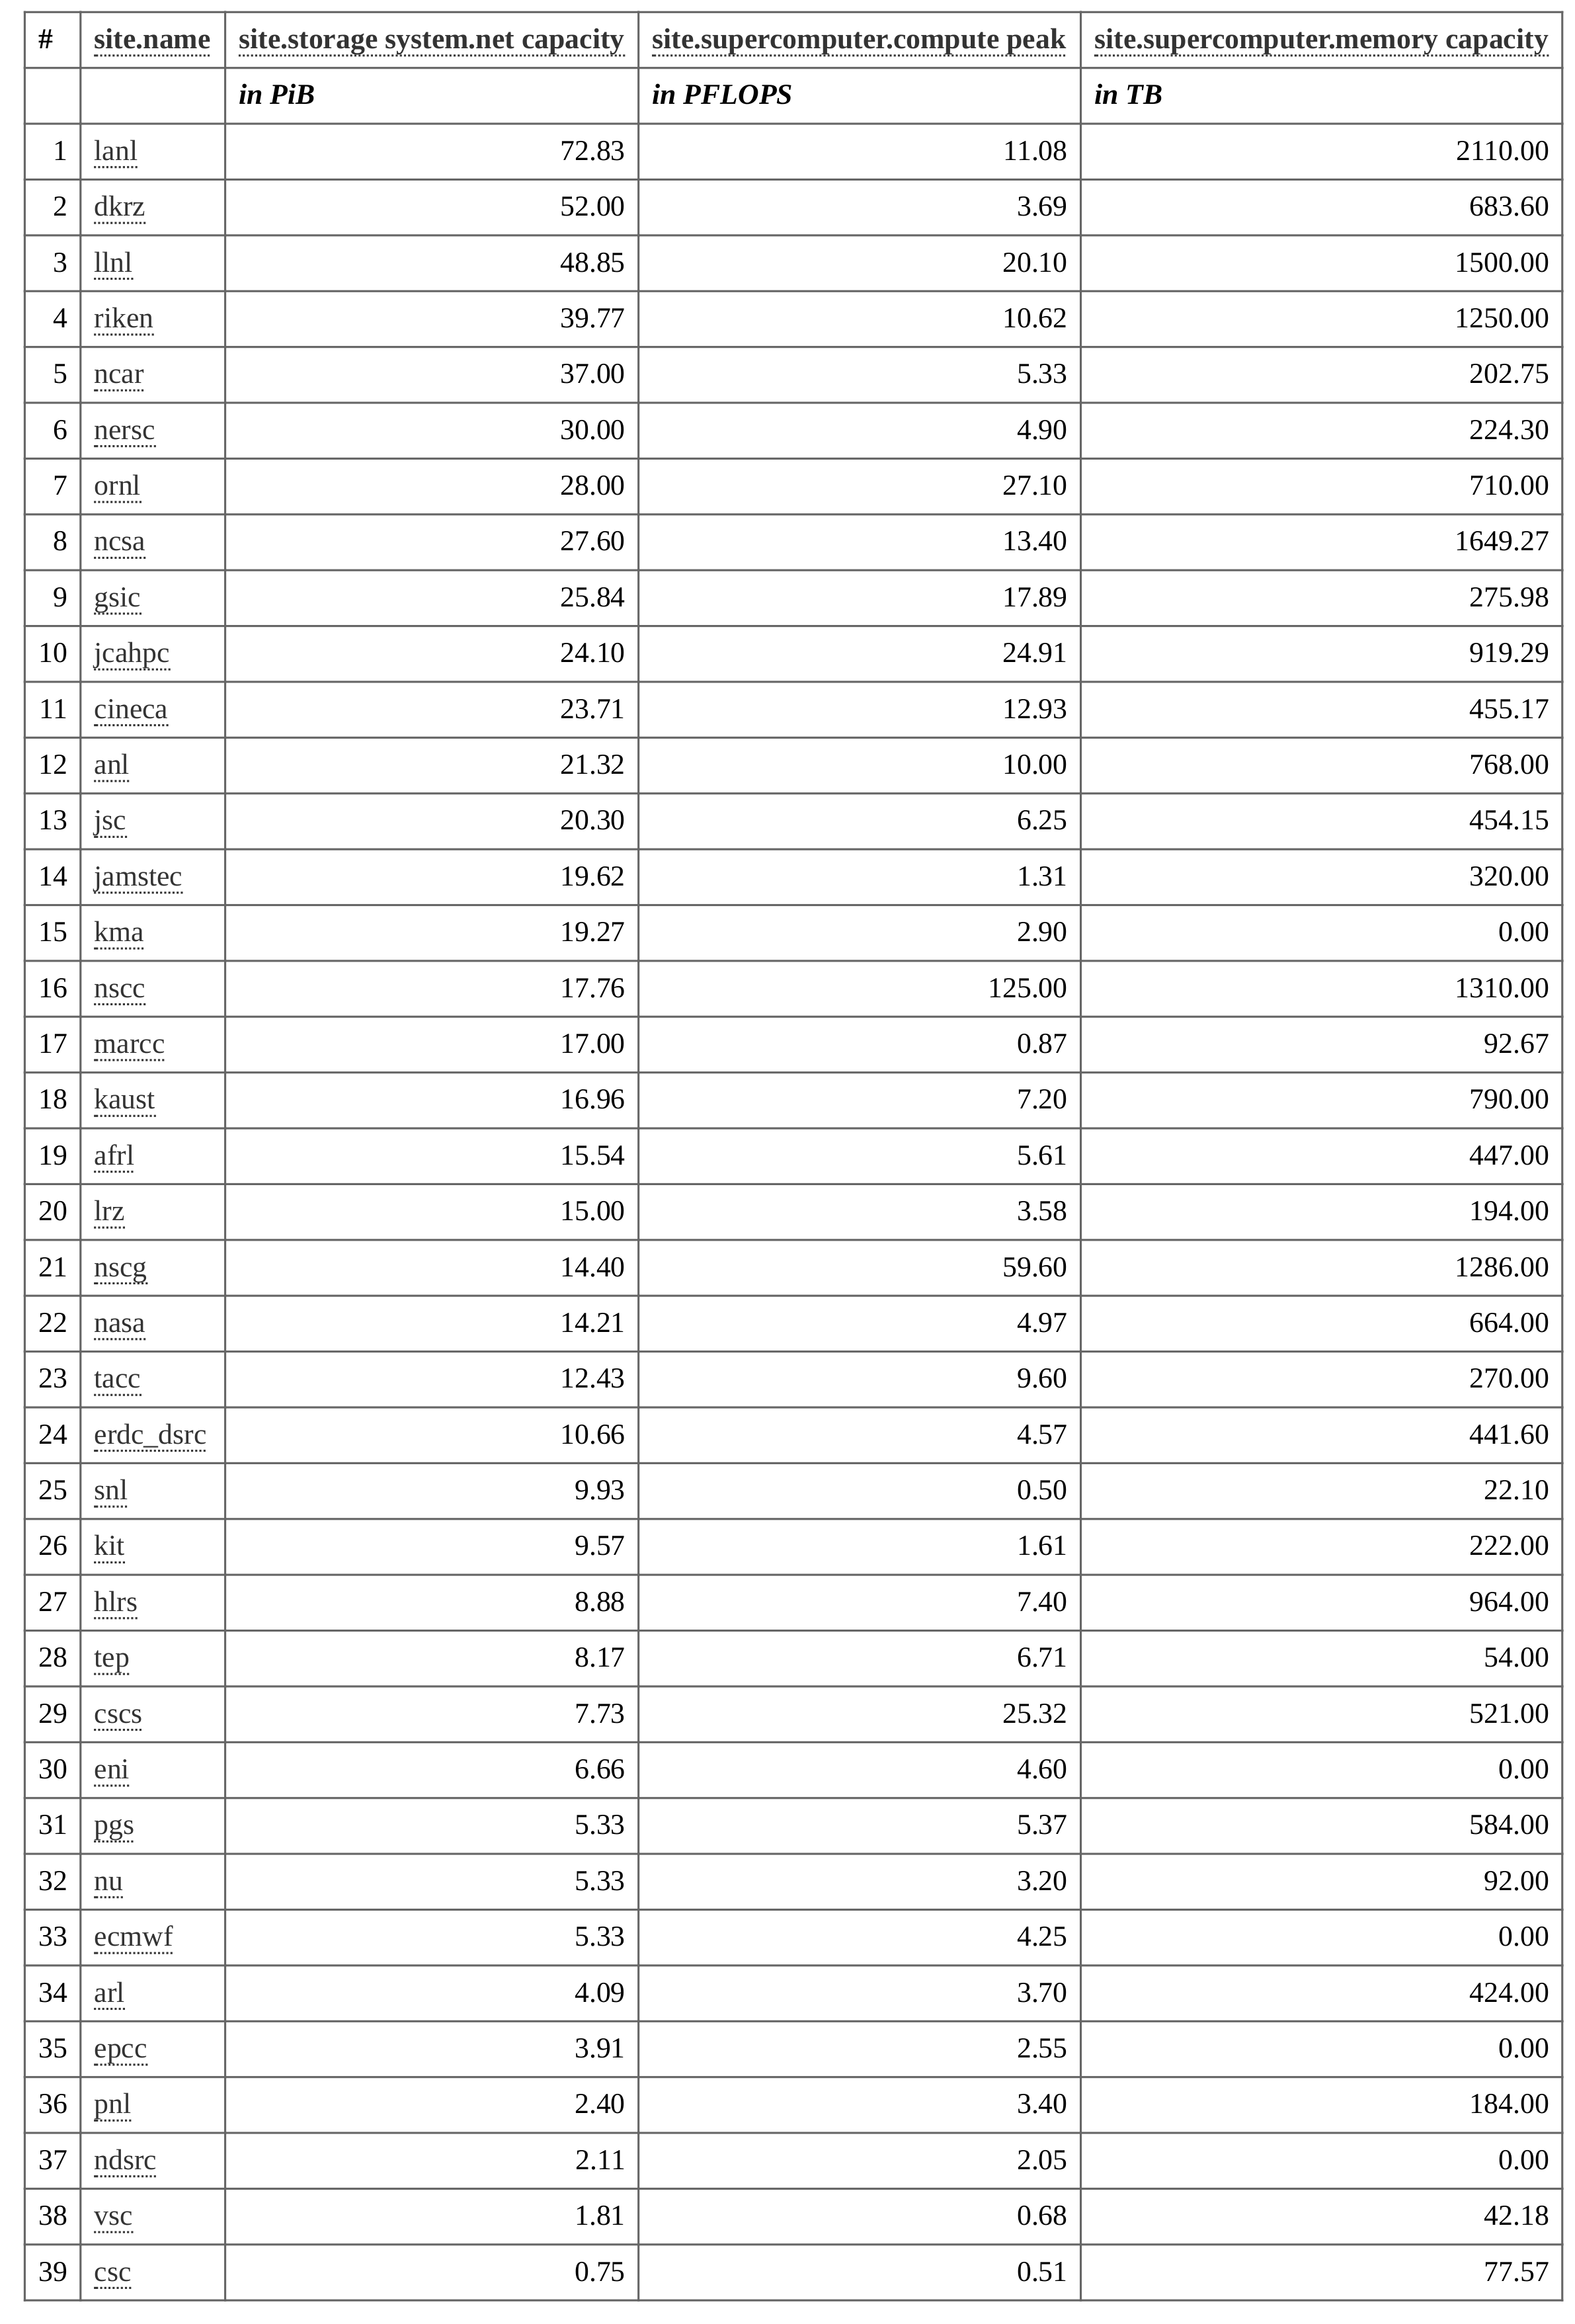
\includegraphics[width=\textwidth]{hpsl-current}


\begin{itemize}\compresslist
\item Various views are possible (subset shown)
\item Supports flexible data aggregation (below)
\end{itemize}

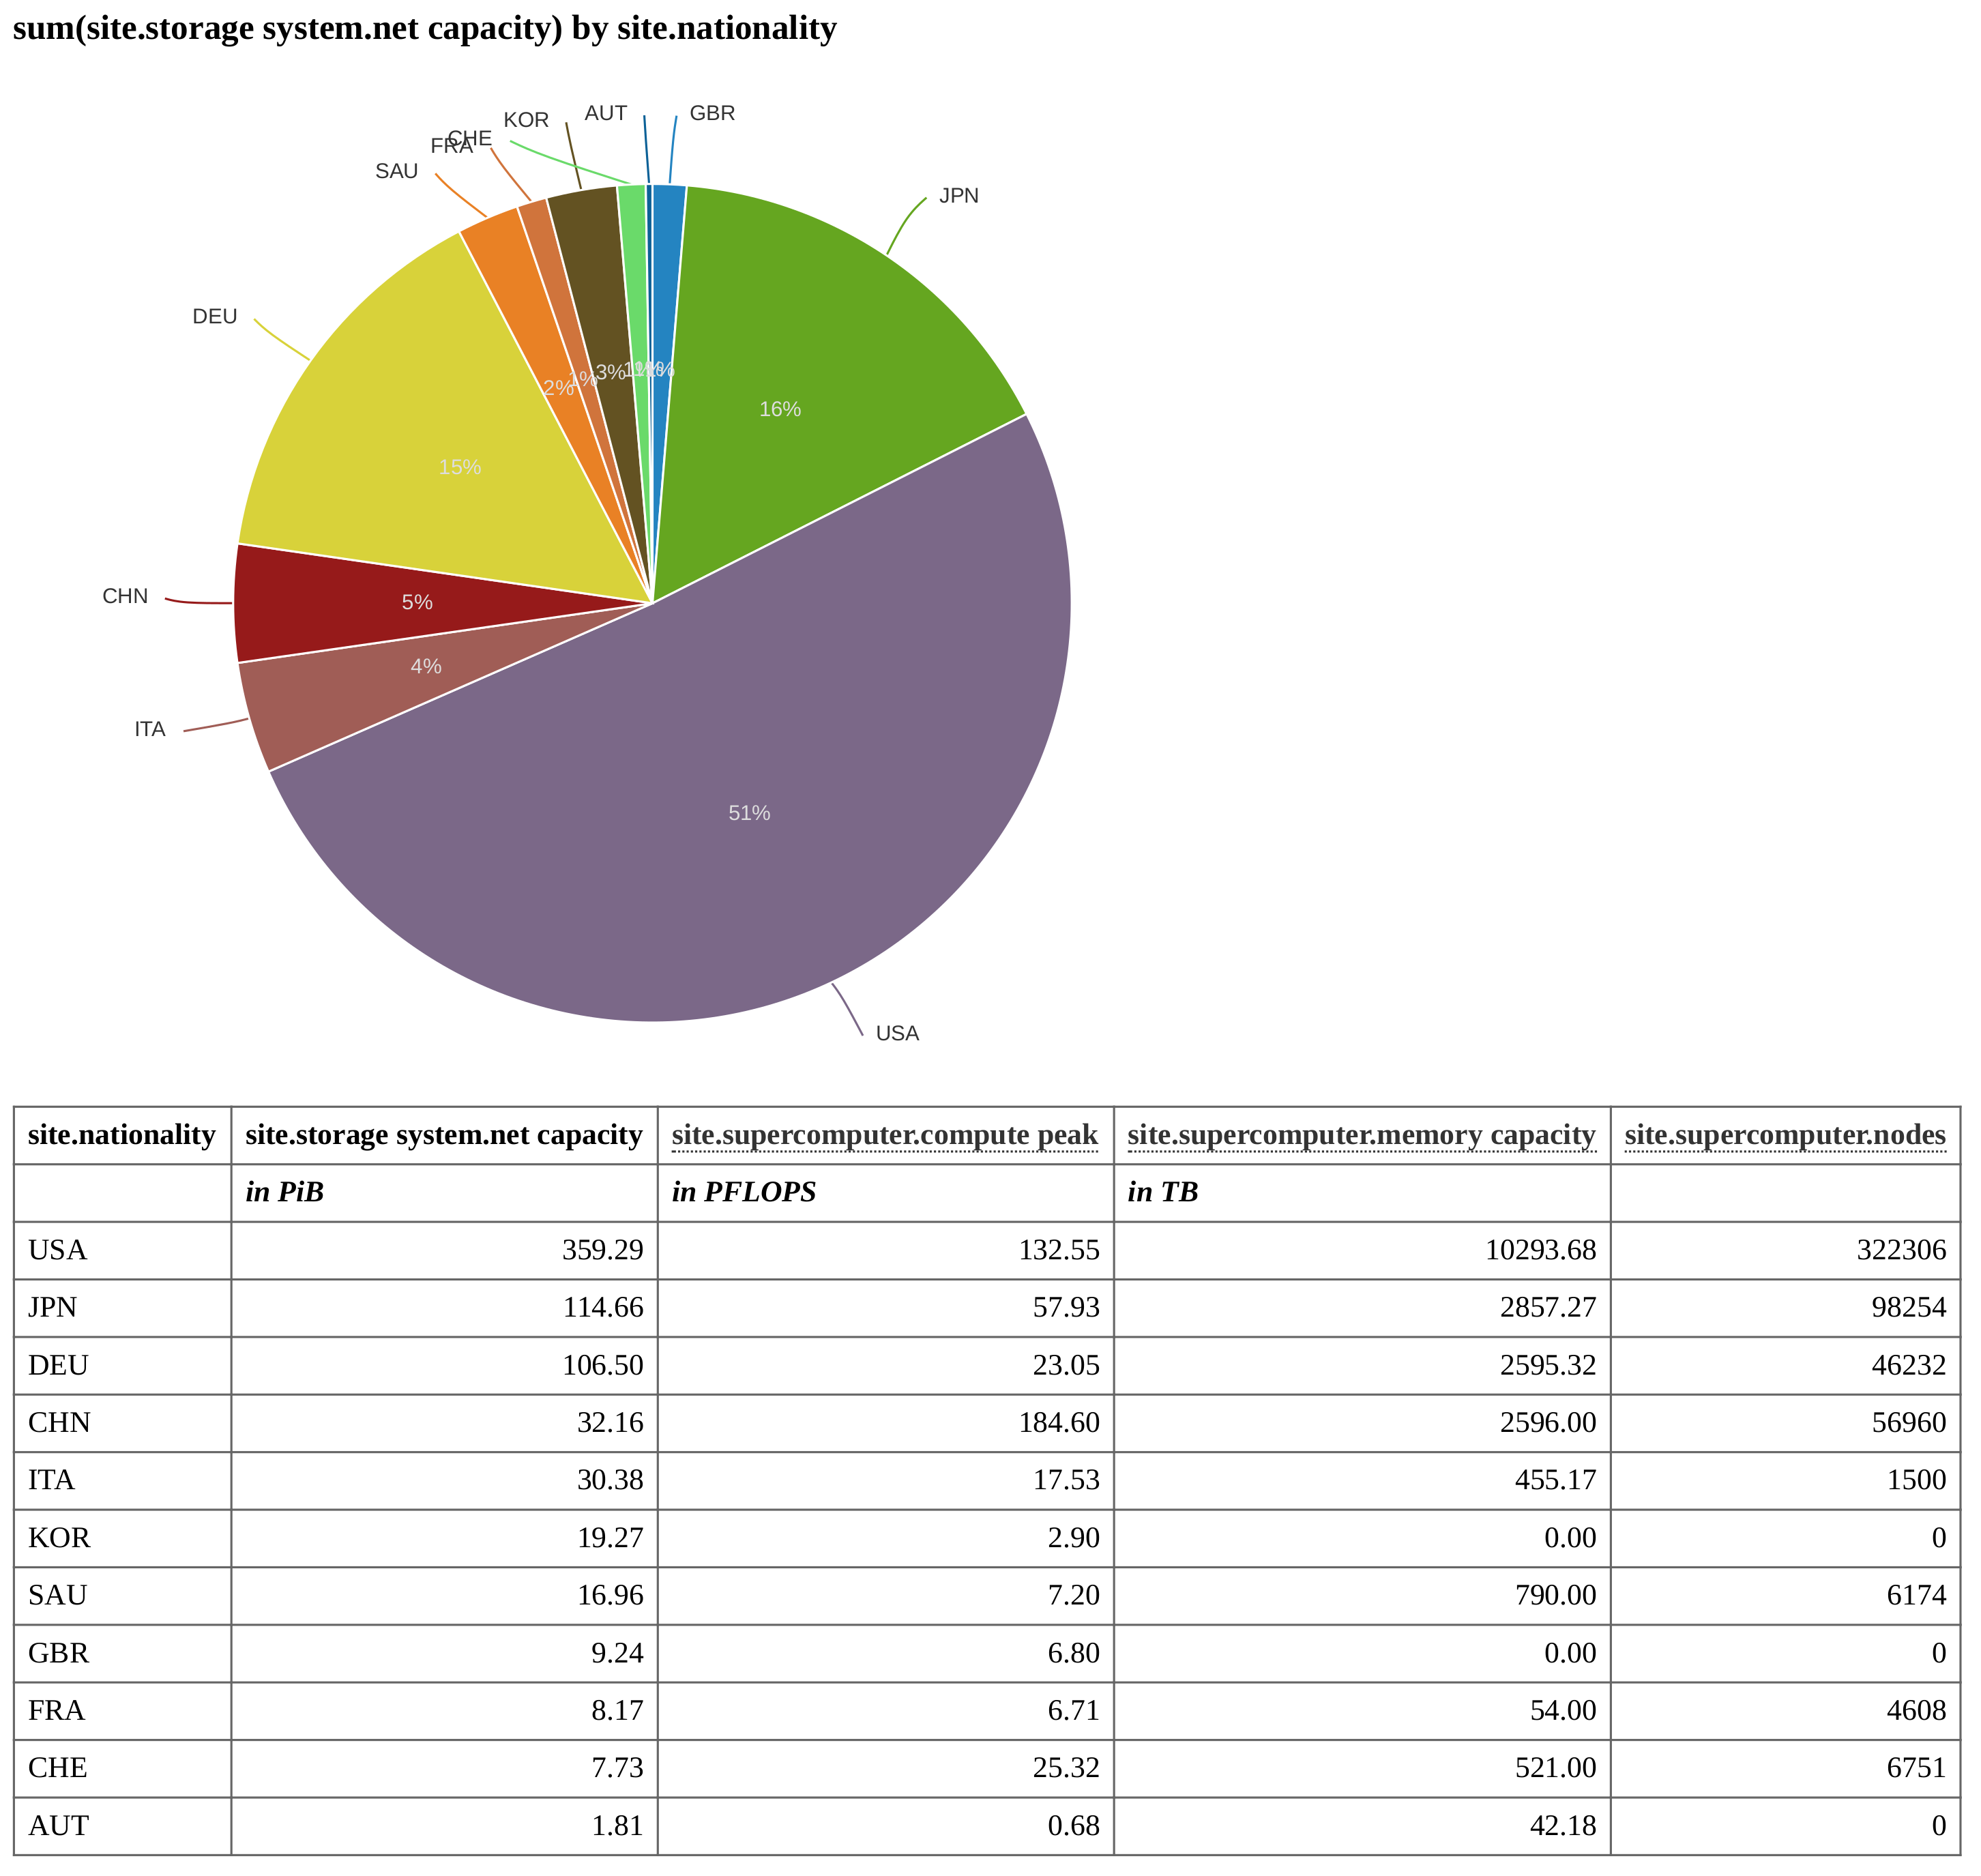
\includegraphics[width=\textwidth]{hpsl-figure}
\end{posterbox}




\begin{posterbox}[name=awareness,column=3,below=engineering]{Derived Analysis}
With the collected data many in-depth analysis becomes possible, for example,
the relationship between storage and memory capacity:

\vspace*{-1em}

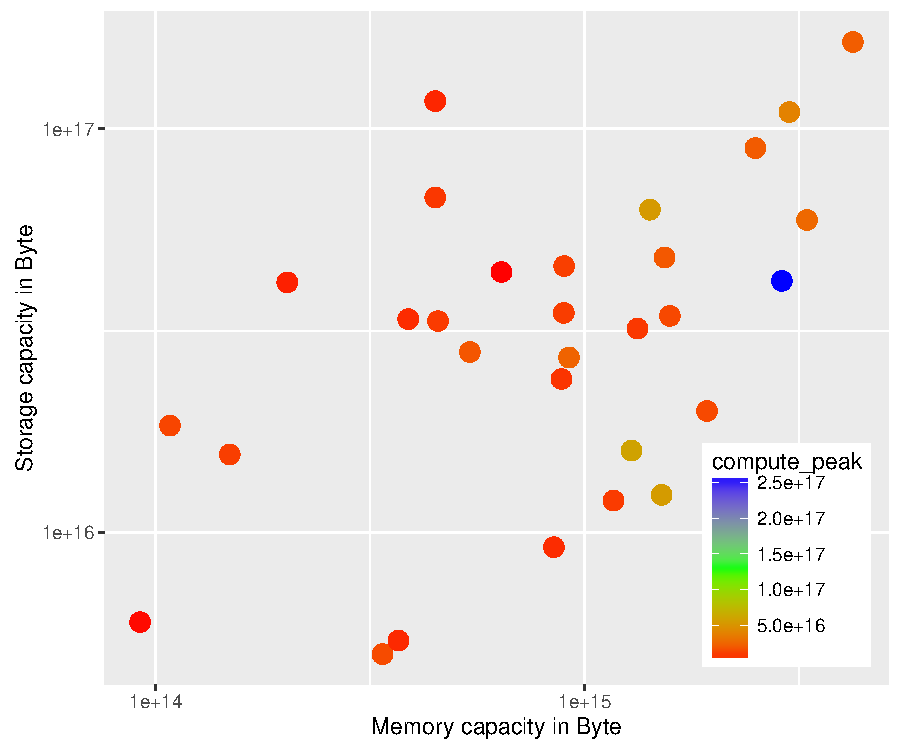
\includegraphics[width=5cm]{memstorage}
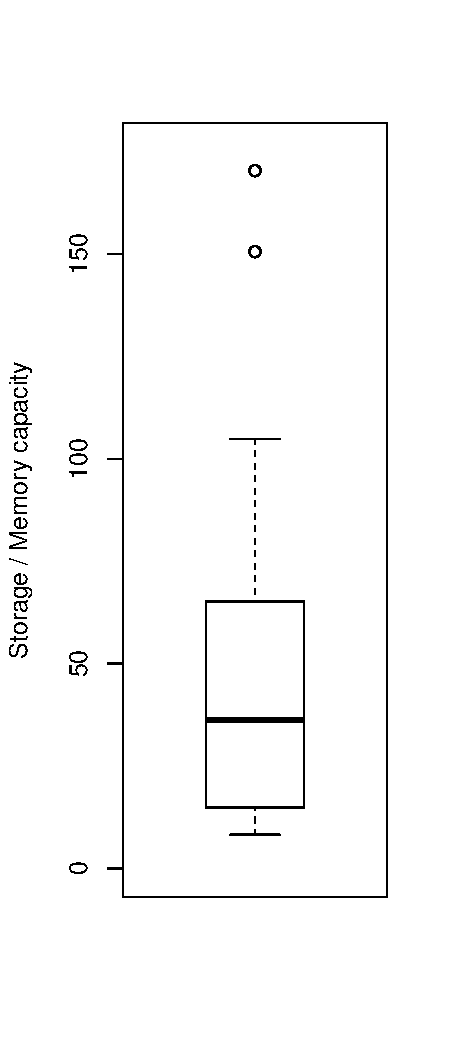
\includegraphics[width=2cm]{capacitymemory}

\vspace*{-2em}
\begin{itemize}\compresslist
\item Correlation storage capacity vs.
  \begin{itemize}\compresslist
  \item memory capacity = 0.63
  \item compute peak = 0.057
  \end{itemize}
\item Mean(storage/mem capacity) = 58
\end{itemize}

\end{posterbox}

\begin{posterbox}[name=b4,column=3,below=awareness]{Ongoing Work}
\begin{itemize}\compresslist
\item Supporting standardization efforts
  \begin{itemize}\compresslist
  \item IO-500 benchmark
  \item Lossy compression interfaces
  \item Data center representation
  \end{itemize}
\item IO-500 agenda:
  \begin{itemize}
  \item June'17, proposal for extension rules
  \end{itemize}
\item Extending schema
\item More HPSL sites
\item Support training and teaching for storage
\end{itemize}
\end{posterbox}


\begin{posterbox}[name=hpccertification,column=3,below=b4, above=bottom]{VI4IO and You}

\begin{minipage}{0.7\textwidth}
Content is under open licenses.
You are welcome to join the mailing lists or participate!
\end{minipage}
\begin{minipage}{0.29\textwidth}

\includegraphics[width=\textwidth]{qr-code.jpg}
\end{minipage}

\vspace*{-0.5em}


\huge \url{https://vi4io.org}
\end{posterbox}


\end{poster}
\end{document}
